%%%%%%%%%%%%%%%%%%%%%%%%%%%%%%%%%%%%%%%%%%%%%%%%%%
%% Allgemeiner Header mit scrreprt				%%
%% Autor: Stefan Zollinger						%%
%% Quellen:	-scrguide							%%		
%%			-www.dante.de						%%
%%%%%%%%%%%%%%%%%%%%%%%%%%%%%%%%%%%%%%%%%%%%%%%%%%

%-------------------------------------------------
%Dokumentklasse und allgemeine Pakete
%-------------------------------------------------
\documentclass[
		11pt, 
		bibliography=totocnumbered,		    %Literaturverzeichnis im Inhaltsverzeichnis 
	  listof=totocnumbered,							%Tab. und Abb.-verzeichnis nummeriert	
		final,												%f�r endversion (draft -> ohne bilder und links, 
		                              %anzeige von Fehlern)
		parskip=half,									%Halbe Zeile Abstand zwischen Abs�tzen.
		twoside=true									%zweiseitig
		]{scrreprt} 	
\usepackage[utf8]{inputenc}
\usepackage{scrhack}					%beseitigt warnung wegen float+koma inkompatibilit�t
\usepackage[T1]{fontenc}			%umlaute als eigene Zeichen
%\usepackage[latin1]{inputenc}	%umlaute erkennen
\usepackage[ngerman]{babel,varioref}
%\usepackage[ngerman]{babel}		%silbentrennung neue deutsche Rechtschreibung
\usepackage{babelbib}					%f�r deutsches literaturverzeichnis
%\usepackage{scrpage2}					%pagestyle
\usepackage{lastpage}					%f�r Referenzen auf letzte Seite
\usepackage{textcomp}					%einige Sonderzeichen
\usepackage{graphicx}	        %grafiken in jpeg,png
\usepackage{epstopdf}		    	%f�r .eps vektorgrafiken
\usepackage{color}						%ben�tigt f�r farbeinstellungen
\usepackage{array}				    %erweiterte Optionen in tabellen (Bsp. ausrichtung innerhalb felder)
\usepackage{subfigure}				%um 2 bilder nebeneinander anzuzeigen
\usepackage{amsmath} 					%mathematischen Textsatz.
\usepackage{amssymb}					%	-Erweiterte math. Sonderzeichen
\usepackage{dsfont}						%	-Mengen			
\usepackage{paralist} 				%kompakte Aufz�hlung: \begin{compactitem}
\usepackage{float}						%f�r H option bei floats(figure,table)
\usepackage{lmodern}					%moderne Schrift
\usepackage{url}				   	 	%korrekte darstellung von urls (mit verlinkung)
\usepackage{changepage}       %f�r adjustwidth auf titelseite
\usepackage{fancyhdr}					%f�r \pagestyle{fancy} -> kopf/fusszeile �ber Textk�rper hinaus
\usepackage{acronym}					%abk�rzungsverzeichnis, Anwendung: \ac{KDE}
\usepackage{cellspace}				%f�r S-operator in Tabellen -> Formeln ber�hren R�nder nicht
\usepackage{booktabs}					%Tabellen: \toprule \midrule \bottomrule
\usepackage{mparhack}         %Repariert falsch gesetzte marginalien am Seitenanfang
\usepackage{setspace}
\usepackage{placeins}

%-------------------------------------------------
% formatierte Listings
%-------------------------------------------------	
\definecolor{commentColor}{rgb}{0.3,0.3,0.3}	%Grau f�r kommentare in Listings
\usepackage{listings}
\lstset{ %
language=Matlab,                % choose the language of the code
basicstyle=\small \ttfamily,    % font style
numbers=none,                   % where to put the line-numbers
numberstyle=\small \ttfamily,      % the size of the fonts that are used for the line-numbers
commentstyle=\color{commentColor},				%kommentare
stepnumber=1,                   % the step between two line-numbers. If it's 1 each line will be numbered
numbersep=5pt,                  % how far the line-numbers are from the code�
xleftmargin=15pt,               % linker rand
xrightmargin=15pt,               % rechter rand
backgroundcolor=\color{white},  % choose the background color. requires \usepackage{color}
showspaces=false,               % show spaces adding particular underscores
showstringspaces=false,         % underline spaces within strings
showtabs=false,                 % show tabs within strings adding particular underscores
frame=lines,  	                  % frame: none|leftline|topline|bottomline|lines|single|shadowboxi
tabsize=2,	                    % sets default tabsize to 2 spaces
captionpos=t,                   % sets the caption-position t/b
breaklines=true,                % sets automatic line breaking
breakatwhitespace=false,        % sets if automatic breaks should only happen at whitespace
escapeinside={\%*}{*)}          % if you want to add a comment within your code
}


%-------------------------------------------------
% Abk�rzungsverzeichnis implementieren
%-------------------------------------------------									
\usepackage{nomencl} 				
\renewcommand{\nomname}{Abkürzungsverzeichnis}
\makenomenclature					%abk.verz. umbenennen

%kommando zum einfachen einstellen der Schrift
% Bsp. \changefont{lmss}{sbc}{n}  %latin modern bold condensed Schriftart der Titel
%      \changefont{lmss}{m}{n}		%latin modern sans serif
\newcommand{\changefont}[3]{\fontfamily{#1}\fontseries{#2}\fontshape{#3}\selectfont}
  
%-------------------------------------------------
% Marginalien/Seitenr�nder
%-------------------------------------------------
\newcommand{\marg}[1]{\marginpar{\raggedright \changefont{lmss}{m}{n} #1}}	
%marginalien linksb�ndig mit \marg{text der marginalie}

%\usepackage[
%			%includemp,				%marginalien in Textk�rper einbeziehen
%			%includeall,
%			%showframe,				%zeigt rahmen zum debuggen		
%			marginparwidth=30mm, 	%breite der marginalien
%			marginparsep=5mm,		%abstand marginalien - text
%			reversemarginpar,		%marginalien links statt rechts
%			left=45mm,				%abstand von Seitenraendern
%			right=25mm,				%
%			top=30mm,
%			bottom=30mm,
%			twoside
%			]{geometry}
			
\usepackage[
			%includemp,				%marginalien in Textk�rper einbeziehen
			%includeall,
			%showframe,				%zeigt rahmen zum debuggen		
			marginparwidth=30mm, 	%breite der marginalien
			marginparsep=5mm,		%abstand marginalien - text
			%reversemarginpar,		%marginalien links statt rechts
			left=25mm,				%abstand von Seitenraendern
			right=45mm,				%
			top=30mm,
			bottom=30mm,
			twoside
			]{geometry}
			
%-------------------------------------------------
%Kopf-/Fusszeile
%-------------------------------------------------
%\pagestyle{scrheadings}
%\clearscrheadfoot															%voreinstellungen l�schen
%\automark[chapter]{chapter}										%Kapitelangabe 
%\ihead{\changefont{lmss}{sbc}{n} \headmark}		%kopfzeile
%\ifoot[																				%fusszeile
%        \changefont{lmss}{m}{n}{ \thepage  /\pageref{LastPage}}]
%        {\changefont{lmss}{m}{n}{ \thepage  /\pageref{LastPage}}}	
        
        
        
%%% Kopf und Fusszeilen
\pagestyle{fancy}					%stil der kopf/fusszeilen 
\renewcommand{\chaptermark}[1]{\markboth{\thechapter.\ #1}{}}	
%damit Kapitelangaben im Header kleingeschrieben werden
\fancyhead{} 						% clear all header fields
\fancyhead[RE,LO]{ \changefont{lmss}{sbc}{n} \leftmark }
\fancyhead[C]{ }
\fancyhead[LE,RO]{ \changefont{lmss}{m}{n} \thepage/\pageref{LastPage} }
%\fancyhead[LO]{\changefont{lmss}{m}{n} \thepage/\pageref{LastPage} \hspace{2.5cm}
%							 \changefont{lmss}{sbc}{n} \leftmark }
\fancyfoot{} 						% clear all footer fields
\fancyfoot[LE,RO]{ }
\fancyfoot[C]{}
\fancyfoot[RE,LO]{  }
\renewcommand{\headrulewidth}{0.5pt}
\renewcommand{\footrulewidth}{0pt}
\fancyhfoffset[LE,RO]{35mm} 			%header und footer nach links verlängern (über marginalien)
\fancypagestyle{plain}{				% plain redefinieren, damit wirklich alle seiten im gleichen stil sind (ausser titlepage)
	\pagestyle{fancy}
}

%-------------------------------------------------
%PDF-Optionen
%-------------------------------------------------
\usepackage[%
	pdftitle={SA},%                                   Titel des PDF Dokuments.
	pdfauthor={Autoren},%                                Autor des PDF Dokuments.
	pdfsubject={Thema},%                                 Thema des PDF Dokuments.
	pdfcreator={LaTeX with hyperref and KOMA-Script},%   Erzeuger des PDF Dokuments.
	pdfkeywords={Schuelsselwrter},%                        auch fr PDF Dokumente indexiert.)
	pdfpagemode=UseOutlines,%                            Inhaltsverzeichnis anzeigen beim ffnen
	pdfdisplaydoctitle=false,%                            Dokumenttitel statt Dateiname anzeigen.
	pdflang=de%                                          Sprache des Dokuments.
]{hyperref}

\definecolor{LinkColor}{rgb}{0,0,0}	%{0,0,0.4} -> Blaue Links im PDF Dokument.
\hypersetup{%
	colorlinks=true,%        Aktivieren von farbigen Links im Dokument (keine Rahmen)
	linkcolor=LinkColor,%    Farbe festlegen.
	citecolor=LinkColor,%    Farbe festlegen.
	filecolor=LinkColor,%    Farbe festlegen.
	menucolor=LinkColor,%    Farbe festlegen.
	urlcolor=LinkColor,%     Farbe von URL's im Dokument.
	bookmarksnumbered=true%  berschriftsnummerierung im PDF Inhalt anzeigen.
}

% bessere float plazierung
\renewcommand{\textfraction}{0.1}
\renewcommand{\topfraction}{0.9}
\renewcommand{\bottomfraction}{0.9}
\renewcommand{\floatpagefraction}{0.35}
\setcounter{totalnumber}{5}

\let\origsection\section{}								%\section sichern als \origsection
\renewcommand{\section}{\FloatBarrier \origsection}		%\section �berschreiben 
														%\FloatBarrier: verhindert, dass Bilder oder Tab. hier weiterrutschen


\begin{document}

\begin{titlepage}

\begin{adjustwidth}{-25mm}{-45mm}
%Seite einmitteln gem�ss werten im geometry package:

\begin{adjustwidth}{60mm}{10mm}
\textsf{
%\textsf{ %sans serif schrift
  \vspace*{2cm}
  \begin{flushleft}
    \huge \textbf{Titel titel titel\\ titel titel titel titel}\\
    \vspace{.25cm}
    \Large untertitel untertitel untertitel untertitel untertitel\\ 
    untertitel untertitel \\
    \end{flushleft}
}
\end{adjustwidth}

\begin{adjustwidth}{35mm}{40mm} 
    \vspace{12cm}
    \large
    \textsf{\textbf{Autoren}}\\
    \textsf{Patrick Fleischmann und Stefan Zollinger}\\
    \textsf{\textbf{Betreuer}}\\
    \textsf{Prof. Dr. Mister X}\\
    \hfill\hbox{}\\
    \textsf{Studienarbeit in \LaTeX-Technik}\\
    \textsf{HSR Hochschule f�r Technik Rapperswil}\\
    \hfill\hbox{}\\
    \textsf{03.09.3033}
\end{adjustwidth}

\end{adjustwidth}

%leere Seite
\newpage                
\thispagestyle{empty}
\mbox{}
\vfill
Dieses Dokument wurde mit \LaTeX \ gesetzt.

\end{titlepage}

\chapter*{Abstract}
\thispagestyle{empty}
Jo do isch dmartina dra was zmache
\begin{itemize}

\item[\textsf{\textbf{\large sadfas asdfsadf asdf}}] \quad \\
Lorem ipsum dolor sit amet, consetetur sadipscing elitr, sed diam nonumy eirmod tempor invidunt ut labore et dolore magna aliquyam erat, sed diam voluptua. At vero eos et accusam et justo duo dolores et ea rebum. Stet clita kasd gubergren

\item[\textsf{\textbf{\large dolores et ea}}] \quad \\
Lorem ipsum dolor sit amet. Lorem ipsum dolor sit amet, consetetur sadipscing elitr, sed diam nonumy eirmod tempor invidunt ut labore et dolore magna aliquyam erat, sed diam voluptua.

\item[\textsf{\textbf{\large sadfas asdfsadf asdf}}] \quad \\
Lorem ipsum dolor sit amet, consetetur sadipscing elitr, sed diam nonumy eirmod tempor invidunt ut labore et dolore magna aliquyam erat, sed diam voluptua. At vero eos et accusam et justo duo dolores et ea rebum. Stet clita kasd gubergren

\item[\textsf{\textbf{\large dolores et ea}}] \quad \\
Lorem ipsum dolor sit amet. Lorem ipsum dolor sit amet, consetetur sadipscing elitr, sed diam nonumy eirmod tempor invidunt ut labore et dolore magna aliquyam erat, sed diam voluptua.

\item[\textsf{\textbf{\large sadfas asdfsadf asdf}}] \quad \\
Lorem ipsum dolor sit amet, consetetur sadipscing elitr, sed diam nonumy eirmod tempor invidunt ut labore et dolore magna aliquyam erat, sed diam voluptua. At vero eos et accusam et justo duo dolores et ea rebum. Stet clita kasd gubergren

\end{itemize}


%leere Seite
\newpage								
\thispagestyle{empty}
\mbox{}

\setcounter{secnumdepth}{2}
\tableofcontents

\chapter{Formelzeichen, Abkürzungen, Definitionen}

\section{Formelzeichen}

\renewcommand{\arraystretch}{1.5}
\begin{table}[!h]
\label{tab:formelzeichen}
\begin{tabular}{l p{9cm} l}
\textbf{Zeichen} & \textbf{Bedeutung} & \textbf{Einheit}  \\ 
  $s_{x, y, z}$ & Momentanpositon in den Raumkoordinaten x, y, z & $	\mathrm{m}$ \\ 
  $a_{x, y, z}$ & $a = \ddot{s}$, Beschleunigung in die Richtungen x, y, z & $ 	\mathrm{\frac{m}{s^2}}$ \\ 
  $\varphi_{x, y, z}$ & Momentan-Winkel, \newline Drehung um x(Roll), y(Pitch), z(Yaw) & $	\mathrm{rad}$ \\ 
  $\omega_{x, y, z}$ & $\omega =  \dot{\varphi}$, Momentan-Winkelgeschwindigkeit um x, y, z & $	\mathrm{\frac{rad}{s}}$ \\ 
  $\alpha_{x, y, z}$ & $\alpha = \ddot{\varphi}$, Rotationsbeschleunigung um x, y, z & $	\mathrm{\frac{rad}{s^2}}$ \\ 
  $F$ & Kraft & $	\mathrm{N}$ \\ 
  $g$ & Erdbeschleunigung ($g \approx 9.81 \mathrm{\frac{m}{s^2}}$) & $	\mathrm{\frac{m}{s^2}}$ \\ 
  $F_G$ & $F_G = m g$, Gewichtskraft & $	\mathrm{N}$ \\ 
  $m_T$ & Totmasse (siehe \ref{sec:definitionen})& $	\mathrm{kg}$ \\
\end{tabular}
\end{table}
\renewcommand{\arraystretch}{1}

\section{Abkürzungen}
\begin{acronym}[FACT] %opt. Argument sollte lüngste Abk. sein
 \acro{DLS}{Dynamic Load Sensor}
 \acro{DMS}{Dehnungs-Messstreifen}
 \acro{FIR}{Finite Impulse Response}
 \acro{TP}{Tiefpass}
 \acro{SICS}{Standard Interface Command Set}
\end{acronym}

\vfill %damit Abkürzungen nicht verrissen werden debug

\section{Definitionen}
\label{sec:definitionen}

\begin{description}
     \item[Wügegut] 
       Gemüss \cite{waegelexikon}: \emph{Bezeichnung für den zu wügenden Gegenstand.}
       
     \item[Kombinierter Schwerpunkt] 
       (auch: Gesamt\-schwer\-punkt) Koordi\-naten des\\ Schwerpunktes eines zusammen\-gesetzten Kürpers. Er berechnet sich als gewichtete Summe der Schwerpunkte der Teilkürper \cite{kuchling}.
              
     \item[Messgewicht]
       Bekanntes Gewicht, das für eine Messung auf die Waage gelegt wurde. 
                     
     \item[Mittelwert]
       Arithmetischer Mittelwert einer Reihe gemüss:
     \begin{equation*}
		 \overline{x} = mean(x) = \frac{1}{N} \sum_{i=1}^N x_i \quad i\in[1,N]
		 \end{equation*}
		 
		 \item[Sample-Standardabweichung]
		   Standard\-abweichung einer Messreihe, berechnet mit dem erwartungs\-treuen Schützer      \cite{mueller}:
		 \begin{equation*}
		 s = std(x) = \sqrt{\frac{1}{N-1} \sum_{i=1}^N (x_i-\bar{x})^2}\quad i\in[1,N]
		 \end{equation*}
		 
		 \item[RMS, Root Mean Square]
		   (auch: Effektivwert)
		 \begin{equation*}
		 x_{RMS} = RMS(x) = \sqrt{\overline{x}^2 + s^2}
		 \end{equation*}
		 Der RMS des Fehlers $RMS(\widehat m - m)$ wird als Vergleichsmass für Kom\-pen\-sations-Methoden verwendet.
		 
		 \item[Justierung]
		  Der Begriff Justierung wird in dieser Arbeit als Synonym zu "`Justierung der Empfindlichkeit"' verwendet. Also gemüss \cite{waegelexikon}: \emph{Das Einstellen der Empfindlichkeit einer Waage mit Hilfe eines Referenzgewichtes.}
		 
		 \item[Wiederholbarkeit]
		 Gemüss \cite{waegelexikon}: \emph{Die Fühigkeit einer Waage, bei mehreren Wügungen des selben Objektes übereinstimmende Messwerte anzuzeigen. Dabei muss die Messreihe unter exakt den selben Bedingungen durchgeführt werden. Die Standardabweichung dieser Messreihe ist ein geeignetes Mass, um den Wert der Wiederholbarkeit anzugeben.}
		 
		\item[Empfindlichkeit]
		Gemüss \cite{waegelexikon}: \emph{ünderung der Ausgangsgrüsse dividiert durch die ünderung der zugehürigen Eingangsgrüsse: $S = \frac{\Delta W}{\Delta m}$. $S$ ist einheitenlos mit dem korrekten Wert 1. Eine Empfindlichkeits-Abweichung führt zu Messabweichungen, welche zum Messgewicht proportional sind.}
		
		\item[Linearitüt]
		Gemüss \cite{waegelexikon}: \emph{Eigenschaft einer Waage, den linearen Zusammenhang zwischen der aufgelegten Last $m$ und dem angezeigten Wügewert $W$ zu folgen.}
		
\end{description}


\chapter{EPS-Grafiken, Listings}
\section{EPS-Grafiken}
\label{sec:epsgrafiken}

EPS-Grafiken (ein Vektorgrafik-Format) werden mit dem epstopdf-Paket automatisch in PDFs umgewandelt, siehe Abb. \ref{fig:yyy}

In \marg{ipsum dolor} 
Lorem ipsum dolor sit amet, consetetur sadipscing elitr, sed diam nonumy eirmod tempor invidunt ut labore et dolore magna aliquyam erat, sed diam voluptua. At vero eos et accusam et justo duo dolores 

Leider \marg{zu tiefe Frequenzen}
dolore magna aliquyam erat, sed diam voluptua. At vero eos et accusam et justo duo dolores et ea rebum. Stet clita kaLorem ipsum dolor sit amet, consetetur sadipscing elitr, sed diam nonumy eirmod tempor invidunt ut labore et dolore magna aliquyam erat, sed diam voluptua. At vero eos et \ref{tab:xxx} accusam et justo duo dolores sd gubergren, no sea  ). Wie in Abb. \ref{fig:yyy} 
\begin{table}[htb]
	\centering
  \caption{TP-Filter Schiff}
	\label{tab:xxx}
	\begin{tabular}{l l}
    \toprule
    Design & Kaiser-Fenster Typ I \\
    \midrule
    $\beta$ & 5.65 \\
    $F_s$ & 91.55Hz \\
    $F_{pass}$ & 0.0001Hz \\
    $F_{stop}$ & 0.05Hz \\ 
    $A_{stop}$ & 60dB \\
    N & 6652 \\		
    \bottomrule
    \end{tabular}
\end{table}
\begin{figure}[htb]%
	\centering
	\includegraphics[width=0.8\textwidth]{pictures/tp_schiff}%
  \caption{ Schrittantwort von TP-Filter}%
	\label{fig:yyy}%
\end{figure}

\pagebreak
Ein \marg{sadfsdaf sdf}
dolore magna aliquyam erat, sed diam voluptua. At vero eos et accusam et justo duo dolores et ea rebum. Stet clita kaLorem ipsum dolor sit amet, consetetur sadipscing elitr, sed diam nonumy eirmod tempor invidunt ut labore et dolore magna aliquyam erat, sed diam voluptua. At vero eos et accusam et justo duo dolores sd gubergren, no sea.

\section{Listings}
Listing \ref{lst:messdaten} benutzt das Listing-Package

\begin{lstlisting}[caption=Ausschnitt aus Messung, label=lst:messdaten]
prozedur bubbleSort( A : Liste sortierbarer Elemente ) 
  n := Luenge( A )
  wiederhole
    vertauscht := falsch
    fuer jedes i von 1 bis n - 1 wiederhole 
      falls A[ i ] > A[ i + 1 ] dann
        vertausche( A[ i ], A[ i + 1 ] )
        vertauscht := wahr
      ende falls
    ende fuer
    n := n - 1
  solange vertauscht und n >= 1
prozedur ende
\end{lstlisting}


\chapter{Grundlagen}
\section{Wügemethoden}
Die \marg{Massevergleich} wohl ülteste und einfachste Wügemethode nennt sich
kompensierender Massevergleich. Dabei wird versucht die gesuchte Masse
müglichst exakt mit bekannten Gewichten zu kompensieren. Als Beispiel für diese Wügemethode sei hier die Balkenwaage erwühnt (Abb. \ref{fig:Federwaage}).

Beim \marg{Federprinzip}
Federprinzip wird die Proportionalitüt zwischen Federweg und Federkraft genutzt:
\begin{equation*}
\frac{F}{s} = k = konst.
\end{equation*}
über diese Beziehung kann von der Auslenkung $s$ auf die Gewichtskraft $F_G$ geschlossen werden. Ist die Erdbeschleunigung $g$ bekannt, kann über $F_G=m g$ schliesslich das Gewicht berechnet werden. \cite{kuchling} Eine Federwaage ist in Abb. \ref{fig:Federwaage} ersichtlich.

\begin{figure}[htb]
	\centering
		\subfigure[Balkenwaage \cite{schulbilder.org}]
			{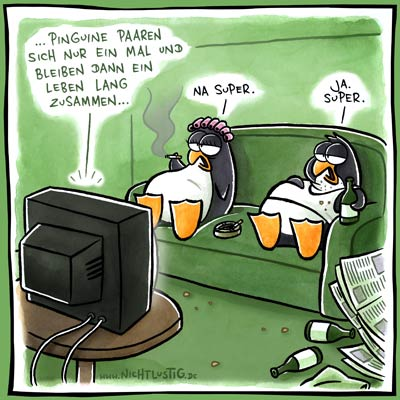
\includegraphics[height=4cm]{./pictures/bild}
			\label{fig:Balkenwaage}}
		\hspace{2cm}
		\subfigure[Federwaage \cite{aaaaaaaaaaa}]
			{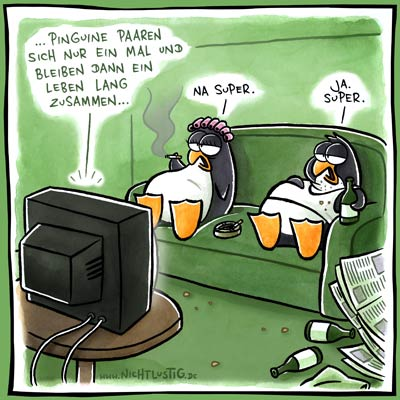
\includegraphics[height=4cm]{./pictures/bild}
			\label{fig:Federwaage}}
		\caption{Balkenwaage und Federwaage}
\end{figure}

Ein \marg{Wügezelle}
sehr weit verbreitetes Wügeprinzip ist die Wügezelle. Hier wird die Verformung eines Federkürpers (i.d.R. aus Metall) mit \ac{DMS} gemessen (siehe Abb. \ref{fig:Federwaage}). \ac{DMS} ündern ihren elektrischen Widerstand, wenn sie verformt werden. Durch geeignete mechanische Konstruktion und Beschaltung kann schliesslich ein zum Gewicht proportionales Signal erzeugt werden. Wügezellen werden in Waagen aller Grüssenordnungen von Haushaltswaagen bis hin zu Kranwaagen eingesetzt.

Für \marg{Doppel-Biegebalken}
kleine Lasten wird der Federkürper einer Wügezelle meist als Doppelbiegebalken ausgeführt. Abb. \ref{fig:Federwaage} zeigt als Beispiel eine solche Wügezelle. Die Doppel\-balken-Konstruktion kann als eine Parallel-Aufhüngung mit vier elastischen Gelenken betrachtet werden. Dadurch kann sich der bewegliche Teil der Wügezelle nur in vertikaler Richtung bewegen und sich nicht neigen. Die Doppelbalken-Wügezelle ist deshalb nur auf Krüfte in vertikaler Richtung empfindlich. Siehe dazu auch \cite{patentYamato}.

\section{asdfsda asdfsd asdfsad}
sadf \marg{sadf s adf asdf }
Lorem ipsum dolor sit amet. Lorem ipsum dolor sit amet, consetetur sadipscing elitr, sed diam nonumy eirmod tempor invidunt ut labore et dolore magna aliquyam erat, sed diam voluptua. At vero eos et accusam  \ref{sec:definitionen}).

\section{asdfsda asdfsd}
sadf \marg{sadf s adf asdf }
Lorem ipsum dolor sit amet. Lorem ipsum dolor sit amet, consetetur sadipscing elitr, sed diam nonumy eirmod tempor invidunt ut labore et dolore magna aliquyam erat, sed diam voluptua. At vero eos et accusam  

Komerziell \marg{sdf sdf asdf}
Lorem ipsum dolor sit amet. Lorem ipsum dolor sit amet, consetetur sadipscing elitr, sed diam nonumy eirmod tempor invidunt ut labore et dolore magna aliquyam erat, sed diam voluptua. At vero eos et accusam  \cite{dynamic}.
 
\section{Titel titel}

Der Begriff dynamische Umgebung bezeichnet eine Situation, \marg{beliebige Bewegungen}
in der das Messsystem beliebigen Bewegungen ausgesetzt ist. Dies ist auf einem Schiff der Fall \cite{comprehensiveMass}. Natörlich werden einige Bewegungsrichtungen störker auftreten als andere. Ein grosses Schiff wird z.B. viel störker um die x-Achse rotieren (Rollen, roll) als um die z-Achse (Gieren, yaw).

Alle \marg{tiefe Frequenzen}
folgenden Betrachtungen beziehen sich auf Bewegungen im Frequenzbereich <10Hz. Auf einem Schiff treten natörlich auch höherfrequente Störungen auf, z.B. Vibrationen des Antriebs. Solche Störungen können aber durch Tiefpass-Filterung bei akzeptabler Zeitverzögerung beseitigt werden.

Wird das Schiff als starrer Körper modelliert, \marg{sechs Freiheitsgrade}
hat die Bewegung im Allgemeinen sechs Freiheitsgrade. Einerseits Translation in den drei Raumdimensionen $s_x, s_y, s_z$, andererseits Drehung oder Rotation um drei unabhöngige Drehachsen $\varphi_x, \varphi_y, \varphi_z$.

För alle folgenden Betrachtungen wird das Messsystem als starrer \marg{starrer Körper}
Körper modelliert. För die Kompensation ist es wichtig, dass die Waagen relativ zu einander feste Positionen haben. Im relevanten Frequenzbereich (<1Hz) ist das Gestell annöhernd ein starrer Körper. Höherfrequente Störeinflösse werden von den Waagen durch ein Tiefpass-Filter unterdröckt. 
\begin{figure}[htb]
	\centering	   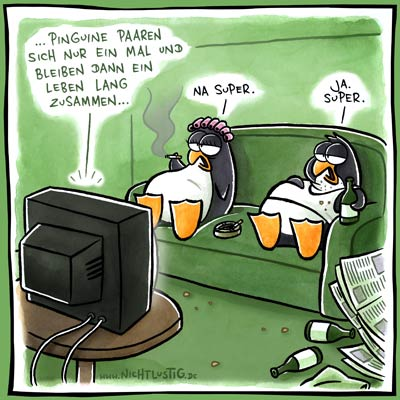
\includegraphics[width=0.5\textwidth]{./pictures/bild}
	\caption{Koordinatensystem auf Schiff}
	\label{fig:koordinatensys_freiheitsgrade}
\end{figure}

\subsection{Beschleunigung durch Translation}

Die Translationsbeschleunigung ist als zweite zeitliche Ableitung des Weges definiert:
\begin{equation*}
a = \ddot{s}
\end{equation*}
Das System kann beliebige Bewegungen in drei \marg{gleiche Beschleunigungen}
Dimensionen ausföhren. Weil es als starrer Körper angenommen wird, sind alle Translationen $s_x, s_y, s,z$ und somit auch Translationsbeschleunigungen $a_{xT}, a_{yT}, a_{zT}$ im ganzen System gleich. Das heisst, alle Waagen erfahren die gleichen Beschleunigungen durch Translationen des Gesam\-mtsystems.

\subsection{Beschleunigung durch Rotation}

\subsubsection{Winkelbeschleunigungen}
Auch Rotationen kann das System in beliebige Richtungen ausföhren. Dies föhrt einerseits zu Winkelbeschleunigungen, andererseits ergeben sich weitere Komponenten der Translationsbeschleunigung. Die Winkelbeschleunigung ist die zweite zeitliche Ableitung des Winkels:
\begin{equation*}
\alpha = \ddot{\varphi}
\end{equation*}
Weil das System ein starrer Körper ist, sind auch die \marg{$\alpha$ öberall gleich}
Winkelbeschleunigungen im ganzen System gleich. Das heisst: Auf alle Waagen wirken die exakt gleichen Winkelbeschleunigungen. 

\subsubsection{Radial- und Tangentialbeschleunigungen}
Rotationen föhren in vom System-Schwerpunkt entfernten \marg{Radial\-beschleunigung}
Punkten zu weiteren Beschleunigungen: Radial- und Tangentialbeschleunigung. Die Radialbeschleunigung $a_r$ wirkt senkrecht zur momentanen Bahngeschwindigkeit. Sie wirkt also in Richtung des Ortsvektors $\vec{r}$. Der Betrag der Radialbeschleunig ist:
\begin{equation*}
a_r = \dot{\varphi}^2 r = \omega^2 r
\end{equation*}
Die Tangentialbeschleunigung  wirkt in Richtung \marg{Tangential\-beschleunigung}
der momentanen Bahngeschwindigkeit eines Objektes. Der Betrag ist:
\begin{equation*}
a_t = \ddot{\varphi} r = \alpha r
\end{equation*}


\listoffigures
\listoftables

\bibliographystyle{gerplain}	%gerplain: [1], geralpha: [Bjar05]
\bibliography{bib/references}

\chapter{Erklärung zur Urheberschaft}
\section*{}
\subsection*{Erklärung}
Ich erkläre hiermit an Eides statt, dass ich die vorliegende Arbeit ohne
Benutzung anderer als der angegebenen Hilfsmittel angefertigt habe; die aus fremden Quellen direkt oder indirekt übernommenen Gedanken sind als solche kenntlich gemacht. Die Arbeit wurde bisher in gleicher oder ühnlicher Form keiner anderen Prüfungsbehürde vorgelegt und auch noch nicht verüffentlicht.

\subsection*{Ort, Datum}
Rapperswil, 18.12.2009

\subsection*{Unterschrift}
Patrick Fleischmann \hspace{3cm} Stefan Zollinger

\appendix
\chapter{Aufgabenstellung}
\label{chp:aufgabenstellung}

\subsection*{Thema:	sadfsdf asdf  asdfsdaf}
\begin{tabular}{ll}
Studenten: & 	Stefan Zollinger, Patrick Fleischmann \\ 
Betreuer: & 	Mister X \\ 
Partner: & 		Firma Y\\ 
\end{tabular}

\subsection*{Kurzbeschreibung}
amet, consetetur sadipscing elitr, sed diam nonumy eirmod tempor invidunt ut labore et dolore magna aliquyam erat, sed diam voluptua. At vero eos et accusam et justo duo dolores sd gubergren, no sea takimata sanctus est Lorem ipsum dolor sit amet.

amet, consetetur sadipscing elitr, sed diam nonumy eirmod tempor invidunt ut labore et dolore magna aliquyam erat, sed diam voluptua. At vero eos et accusam et justo duo dolores sd gubergren, no sea takimata sanctus est Lorem ipsum dolor sit amet.

\subsection*{Aufgabenstellung}
\begin{itemize}
	\item sdf sadf dssadf 
	\item asdf sadfsa asdfsd sadf 
	\item asdf asdfasd f asdf
	\item Aasdf asdfasd fas df
\end{itemize}

\subsection*{Erwartete Ergebnisse}
\begin{itemize}
	\item asdfasd fasdfsadfasdfsdafsdsd sadf sdaf
	\item sadfsadf asdfasd asdf 
\end{itemize}








\end{document}





